\documentclass[letter, 10pt]{article}
\usepackage[utf8]{inputenc}
\usepackage[spanish]{babel}
\usepackage{amsfonts}
\usepackage{amsmath}
\usepackage[dvips]{graphicx}
\usepackage{url}
\usepackage[top=3cm,bottom=3cm,left=3.5cm,right=3.5cm,footskip=1.5cm,headheight=1.5cm,headsep=.5cm,textheight=3cm]{geometry}
\usepackage{listings}
\usepackage{color}
\usepackage{fancyvrb}
\usepackage{fancyhdr}

\pagestyle{fancyplain}

\lhead{Workshop Taller de Gestión} %Parte superior izquierda
\rhead{\bf \it Tutoriales} %Parte superior derecha
\lfoot{} %Parte inferior izquierda.
\cfoot{} %Parte inferior central
\rfoot{\bf \thepage} %Parte inferior derecha
\renewcommand{\footrulewidth}{0.4pt} %Linea de separacion inferior


\begin{document}

\title{Tutorial Skype}
\author{Rodrigo Fernández \and Cristián Maureira \and Gabriel Zamora\\ \small{\texttt{\{rfernand,cmaureir,gzamora\}@inf.utfsm.cl}}}
%\titlegraphic{
\includegraphics[height=1cm]{img/logos}}
\date{\today}

\maketitle

\section{Qué es Skype}

Skype es un software para realizar llamadas sobre Internet (VoIP). Permite comunicación entre computadores y teléfonos fijos, mediante el uso de créditos. También soporta comunicación mediante video y conferencias entre varias personas.

\section{Instrucciones de uso}

\subsection{Preliminares}

\begin{itemize}
	\item Descargar cliente Skype
	\item Crear cuenta Skype
	\item Agregar contactos
\end{itemize}

\subsection{Conferencias}

Debido a que las conferencias se realizan entre varias personas en un mismo lugar, se hace indispensable la utilización de dispositivos que faciliten dicha tarea, por lo que 
contar con un hardware especializado para ello, permite establecer comunicaciones acorde a lo planeado.

Para dicho propósito usualmente se utiliza un dispositivo denominado Voice Station, el cual realiza la tarea de reproducir sonido e interpretarlo (micrófono), además de permitir marcado telefónico, por lo que mediante una pequeña configuración con un computador, más el agregado de poseer una cuenta Skype para marcado internacional, puede reemplazar perfectamente el uso de un teléfono común y corriente.

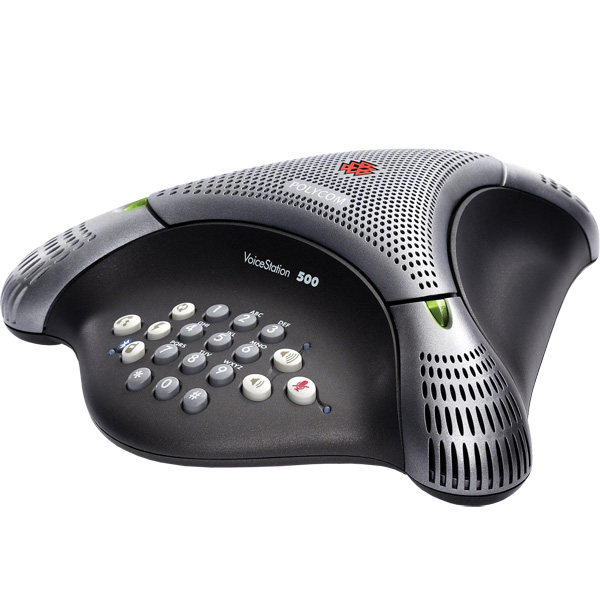
\includegraphics[scale=0.4]{img/voicestation}

\section{Ejercicio}

Por último, intentaremos establecer una conferencia mediante la utilización de audio, entre 2 o más participantes.

\begin{enumerate}
	\item Abrir cliente Skype
	\item Crear cuenta de usuario
	\item Agregar a otros usarios
	\item Establecer una pequeña conferencia (audio)
\end{enumerate}

\end{document}
